
% \documentclass[blackref,approvalform,dvipsnames]{drexel-thesis}
\documentclass[draft,dvipsnames]{drexel-thesis}


\author{Jae Hoon Kim}
\title{Classifying Human Driving Behavior via Deep Neural Networks}
\DUTmonth{June}
\DUTyear{2017}
\degree{Master in Computer Science}
\advisor{Santiago~Onta\~{n}\'{o}n, Ph.D.}
\copyrighttext{\copyrighttextCCBYSA}

\usepackage[numbers,sort&compress]{natbib} % fancy citation extensions
\bibliographystyle{unsrtnat}


% \usepackage{fancyvrb} % nicer verbatim handling
% \DefineShortVerb{\|}  % \verb+TEXT+  ->  |TEXT|

\usepackage{xcolor}
\usepackage{colortbl,booktabs}
\usepackage{xspace}
\usepackage{multirow}
\usepackage{wrapfig} % text around figures
\usepackage{amssymb} % \mathbbstarcra
\usepackage[final]{listings} % algorithms formated in code
\usepackage{enumitem} % compact imte lists
\usepackage{subcaption} % for subfigure (figures side-by-side)
\usepackage{mathtools}
\usepackage{soul}
\usepackage[detect-all]{siunitx} % Aligning numbers by decimal points in table columns

\usepackage{algorithm, soul}
\usepackage[noend]{algpseudocode}
\algnewcommand{\Break}{\textbf{break}}

\newcommand{\todo}[1]{{\color{red}{\tt #1}}}
% \newcommand{\toredo}[1]{{\leavevmode\color{Plum}#1}}
\newcommand{\toredo}[1]{#1}
\newcommand{\modified}[1]{{\leavevmode\color{blue}#1}}
% \newcommand{\modified}[1]{#1}
\newcommand{\highest}[1]{\textcolor{Maroon}{\textbf{#1}}}
\newcommand{\StarCraft}{\mbox{\textsc{StarCraft}}\xspace}
\newcommand{\BroodWar}{\textsc{StarCraft: Brood War}\xspace}
\newcommand{\WarCraft}{\mbox{\textsc{WarCraft}}\xspace}
\newcommand{\WarCraftII}{\mbox{\textsc{WarCraft II}}\xspace}
\newcommand{\WarCraftIII}{\mbox{\textsc{WarCraft III}}\xspace}
\newcommand{\Wargus}{\mbox{\textsc{Wargus}}\xspace}
\newcommand{\Spring}{\mbox{\textsc{Spring}}\xspace}
\newcommand{\BWTA}{\textsc{BWTA}\xspace}
\newcommand{\BWTAb}{\textsc{BWTA2}\xspace}
\newcommand{\BWAPI}{\textsc{BWAPI}\xspace}
\newcommand{\SparCraft}{\textsc{SparCraft}\xspace}
\newcommand{\Lanchester}{\mbox{\emph{TS-Lanchester}$^2$}\xspace}
\newcommand{\cop}{\textsc{COP}\xspace}
\newcommand{\Ghost}{\textsc{GHOST}\xspace}
\newcommand{\Nova}{\textsc{Nova}\xspace}




\begin{document}
\begin{preamble}

% \begin{dedications}
% We're in \iffinal{final}{draft} mode!
% \end{dedications}

% \begin{acknowledgments}
% bla bla bla
% \end{acknowledgments}

\tableofcontents
\listoftables
\listoffigures

% \iffinal{}{\newpage}

\begin{abstract}
The average person spends several hours a day behind the wheel of their vehicles, which are usually equipped with on-board computers capable of collecting real-time data concerning driving behavior. However, this data source has rarely been tapped for healthcare and behavioral research purposes. This MS thesis is done in the context of the {\em Diagnostic Driving} project, an NSF funded collaborative project between Drexel, Children Hospital of Philadelphia (CHOP) and the University of Central Florida that aims at studying the possibility of using driving behavior data to diagnose medical conditions. 
%
Specifically, this paper introduces focuses on the classification of driving behavior data collected in a driving simulator using deep neural networks. The target classification task is to differentiate novice versus expert drivers. The paper presents a comparative study on using different variants of LSTM (Long-Short Term Memory networks) and Auto-encoder networks to deal with the fact that we have a small amount of labels (16 examples of people driving in the simulator, each labeled with an ``expert'' or ``inexpert'' label), but each simulator drive is high dimensional and too densely sampled (each drive consists of 100 variables sampled at 60Hz).
%
Our results show that using an intermediate number of neurons in the LSTM networks and using data filtering (only considering one out of each 10 samples) obtains better results, and that using Auto-encoders works worse than using manual feature selection.
\end{abstract}
\end{preamble}

\begin{thesis}



% ####################################################################################################################################
\chapter{Introduction}\label{chap:intro}
% ####################################################################################################################################

Introduction Section
\begin{enumerate}
\item Problem Statement
\end{enumerate}



% ====================================================================================================================================
% ====================================================================================================================================
\chapter{Background}\label{sec:bg}
% ====================================================================================================================================
% ====================================================================================================================================
This chapter presents the necessary background to understand the experiments presented later in the paper. This chapter is dived to three sections. First Section \ref{sec:DL} covers basic deep learning including recurrent neural network and auto-encoder. Second Section \ref{sec:DLL} compares deep learning libraries: DL4J, Theano, and Tensorflow. The last Section \ref{sec:MLDD} introduces current trend of machine learning with driving data.

\section{Deep Learning}\label{sec:DL}
This section covers basic concept of deep learning. First Subsection \ref{subsec:basicDL} introduces to deep learning, and next Section \ref{subsec:RNN} deals with recurrent neural network and long short term memory neural network. The last Subsection \ref{subsec:AE} covers auto-encoders.

\subsection{Basic Concepts}\label{subsec:basicDL}
{\color{blue} This part Explain basic deep learning [...]}

\subsection{Recurrent Neural Network}\label{subsec:RNN}

\begin{enumerate}
\item Basic concepts of recurrent neural networks:

	A recurrent neural network (RNN) is a neural network that is specialized for processing a sequence of input values \cite{Goodfellow-et-al-2016}. Figure \ref{fig:RNN} illustrates abstract structure of RNN. RNN has two input. One input is from data such as normal neural network input but another input is from previous output. The property gives benefit for sequential input data. This is because past output affects to current output. With sequential data, previous data can affect to current data and RNN considers previous output for current output. It means that even input from data are equal if previous output are different, current output are also different.
	
\begin{figure}[t!]
    \centering
    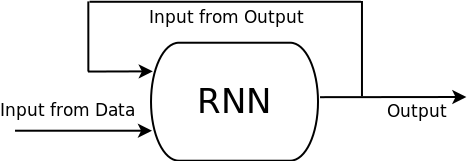
\includegraphics[width=0.65\textwidth]{pictures/figures/RNN.png}
    \caption{RNN}
    \label{fig:RNN}
\end{figure}
	
	For example, human language sentences have series of words and meaning of words is different in different context. RNN can be used for that. Another example is driving data which is used later on the paper.  Driving data are multi-dimension data with time domain. RNN can be used for the data because it is sequential data with time domain.
	
	To describe RNN in math equation, let $\vec{x^t} = \{ x_1^t, ..., x_n^t\} \in \mathbb{R}^n$ be a vector that represents the input data at time $t$, $\vec{h^t} = \{ h_1^t, ..., h_m^t\} \in \mathbb{R}^m$ be result from hidden layer on time $t$, and $\vec{o^t} = \{ o_1^t, ..., o_l^t\} \in \mathbb{R}^l$ be output on time $t$. For transform matrix, let $\bold{U}: \mathbb{R}^n \rightarrow \mathbb{R}^m$ be a transform matrix for input data, $\bold{V}: \mathbb{R}^m \rightarrow \mathbb{R}^l$ be a transform matrix for data from hidden layer, and $\bold{W}: \mathbb{R}^l \rightarrow \mathbb{R}^m$ be a transform matrix for previous output. The figure \ref{fig:unfold_RNN} illustrates unfolded RNN with defined symbols. The result from hidden layer can be calculated by 
	$$\vec{h^t} = \bold{f}(\vec{x^t}\bold{U} + \vec{o^{t-1}}\bold{W} + \vec{b_h})$$ where $\bold{f}()$ is activation function for hidden layer and it is applied for each elements in given vector, $\vec{b_h} \in \mathbb{R}^m$ is a vector for hidden layer bias. Then the output can be calculated by
	$$\vec{o^t} = \bold{g}(\vec{h^t}\bold{V}+\vec{b_o})$$ where $\bold{g}()$ is activation function for output layer and it is applied for each elements in given vector, $\vec{b_o} \in \mathbb{R}^l$ is a vector for output layer bias. Therefore, RNN can be written in
	$$\vec{o^t} = \bold{g}(\bold{f}(\vec{x^t}\bold{U} + \vec{o^{t-1}}\bold{W} + \vec{b_h})\bold{V}+\vec{b_o})$$
	
\begin{figure}[t!]
    \centering
    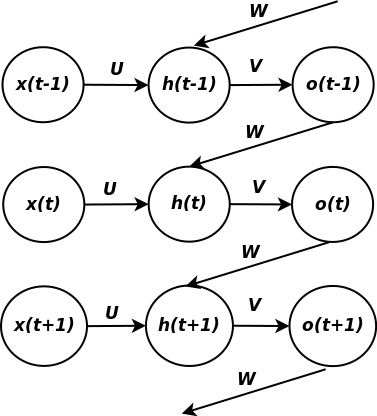
\includegraphics[width=0.5\textwidth]{pictures/figures/unfold_RNN.png}
    \caption{Unfold RNN {\color{red} change variables}}
    \label{fig:unfold_RNN}
\end{figure}

	RNN is not always like the Figure \ref{fig:unfold_RNN}. Input from previous output can be replaced by result of previous hidden layer. The main idea of RNN is when neural network decides current output it considers previous state.
	

\item Long Short Term Memory (LSTM) networks:

	Basic RNN has the problems of long term dependency. When RNN passes previous output for current output, some information in the input might not need or might need for future. RNN does not have ability to filter unnecessary information or to store necessary information. Long Short Term Memory (LSTM) neural network can handle these problems.
	
	LSTM is a type of RNN and introduced by Hochreiter and Schmidhuber \cite{hochreiter1997long}. LSTM solves long term dependency problems in RNN by memory cells. LSTM manages memory cells as storage of knowledge. LSTM filters unnecessary information from memory cells and records necessary information on memory cells.
	
	The structure of LSTM consists of four gates: forget gate, input gate, input modulation gate, and output gate. Each gates have different purpose and Christopher Olah's blog \footnote{\url{http://colah.github.io/posts/2015-08-Understanding-LSTMs}} develops an intuition for concept of LSTM and explains purpose of each gates. The paper \cite{zaremba2014recurrent}  describes LSTM in mathematical term. Let us first provide an intuitive description of how LSTM work by following Christopher Olah's blog, before providing a more in-depth formalization.
	
%	and the paper \cite{zaremba2014recurrent} 
	
%	Bengio mentioned on his paper \cite{bengio2009learning} that each layers in deep neural network should have {\color{red} a} purpose. LSTM can be divided to four layers: forget gate, input gate, input modulation gate, and output gate. Each layers have different purpose {\color{red} [santi: this paragraph does not flow very well], even if Bengio mentioned it, why is it important? you need to explain WHY is it that each layer should have a purpose. Otherwise, we just have to blindly believe in Bengio :)}.

%	 Colah's blog \footnote{\url{http://colah.github.io/posts/2015-08-Understanding-LSTMs}} develops an intuition for concept of LSTM and explains purpose of each layer{\color{red} \st{s}}. The paper \cite{zaremba2014recurrent} describes LSTM in mathematical term{\color{red}s}. In this paper, I'm going to summarize both the Colah's blog and the paper \cite{zaremba2014recurrent}
	
	\begin{enumerate}
	\item An intuitive explanation of LSTMs:
	
		The easiest way to understand LSTM is to understand memory cell and purpose of four different gates. Memory cell makes LSTM different from RNN. Memory cell stores important information and filters unimportant information for future. Three of four gates are involved in the memory cells to store and filter information.
		
		The first gate affecting to memory cells is forget gate. The forget gate decides unnecessary data from input data and previous output then applies it to memory cells. Other two gates are input gate and input modulation gate and these also affect to memory cells. The two gates decide what information remember then apply it to memory cells. The last gate is output gate and it does not directly affect to memory cells. Output gate also has two inputs from input data and previous output, and output from output gate is multiplied by memory cells to make final output. The Figure \ref{fig:LSTM} illustrates LSTM neural network with four gates and next part describes more detail of LSTM and the figure in mathematical terms.

\begin{figure}[t!]
    \centering
    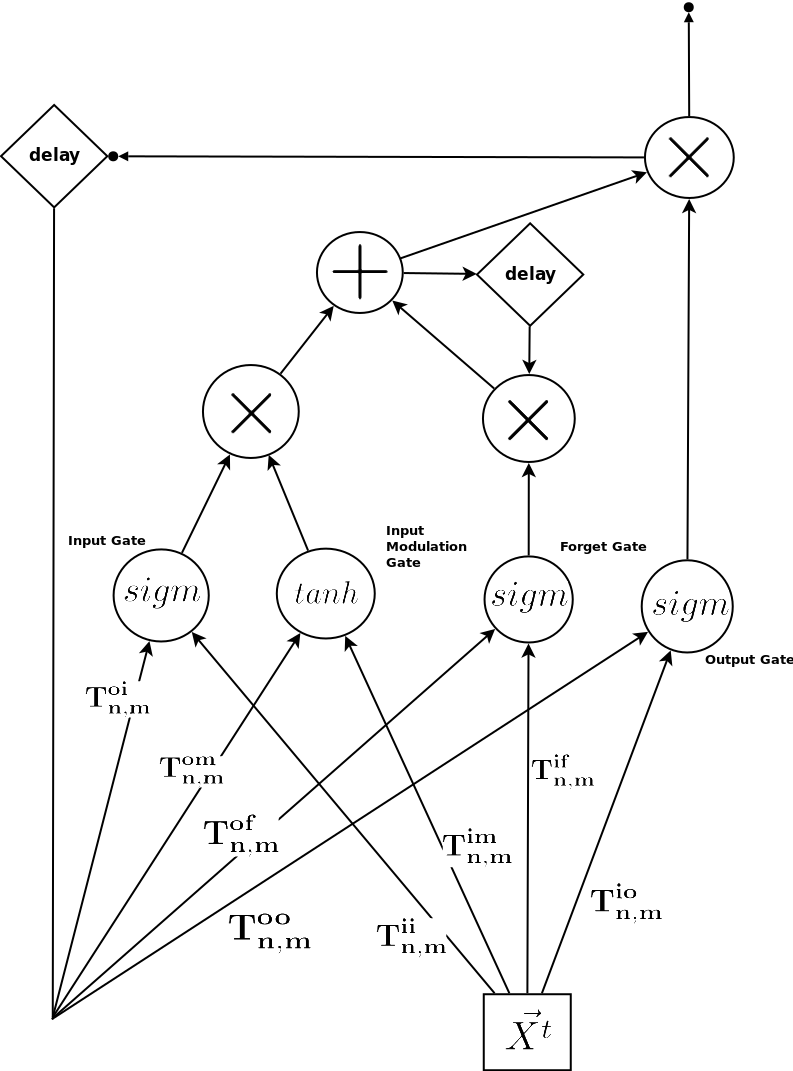
\includegraphics[width=0.75\textwidth]{pictures/figures/LSTM.png}
    \caption{LSTM {\color{red} change variables}}
    \label{fig:LSTM}
\end{figure}
		
		% It consists of sigmod {\color{red} [santi: instead of saying ``It consists of sigmod'', you should say something like ``The units in this layer use a sigmoid activation function'' (same comment for all the other layers below)]} layer with previous output and current input data {\color{red} [santi: a reader not familiar with LSTMs will not know what is ``previous output'' or ``current input'', so you need a figure that explains it]}. The result of the forget gate is multiplied by previous cell state to build current cell state.
		
		% The second layer is input gate and also consists of sigmod layer with previous output and current input data. The result of the input gate is multiplied by the result of input modulation gate then it affects to cell state {\color{red} [santi: all of these terms should appear in a figure, otherwise, a reader not familiar with it will not understand what you are saying. But also, even if you have a figure, you need to explain what each term is, e.g., explain what is ``input modulation'', what is ``cell state'', etc.]}. The meaning of input gate is to decide{\color{red} \st{s}} what data to remember.
		
		% The third layer is input modulation gate. It consists of tanh with previous output and current input. It is multiplied by the result of second layer and affects to current cell state.
		
		% The last layer is output gate. The layer decides what data should be passed to current output from previous output and current input. the output gate also consists of sigmoid with two inputs: last output and current input. The result of the layer is multiplied by current cell state passed tanh.
	
	\item Modeling LSTMs in mathematical terms:
	
		To describe LSTM in mathematical terms, let $\vec{x^t} = \{ x_1^t, ..., x_n^t\} \in \mathbb{R}^n$ be a vector that represents the input data at time $t$, $\vec{i^t} = \{i_1^t, ..., i_m^t\} \in \mathbb{R}^m$ be result from input gate on time $t$, $\vec{m^t} = \{m_1^t, ..., m_m^t\} \in \mathbb{R}^m$ be result from input modulation gate on time $t$, $\vec{f^t} = \{f_1^t, ..., f_m^t\} \in \mathbb{R}^m$ be result from forget gate on time $t$, $\vec{o^t} = \{o_1^t, ..., o_m^t\} \in \mathbb{R}^m$ be result from output gate on time $t$, $\vec{c^t} = \{c_1^t, ..., c_m^t\} \in \mathbb{R}^m$ be memory cells on time $t$, and $\vec{h^t} = \{h_1^t, ..., h_m^t\} \in \mathbb{R}^m$ be final result on time $t$.
Each gates have transform matrices for inputs. Let $\bold{T_{n,m}}: \mathbb{R}^n \rightarrow \mathbb{R}^m$ be a transform matrix from $n$ dimension to $m$ dimension. Let $\bold{T_{n,m}^{ii}}$ be a transform matrix for input from data in input gate, $\bold{T_{m,m}^{oi}}$ be a transform matrix for input from previous output in input gate, $\bold{T_{n,m}^{im}}$ be a transform matrix for input from data in input modulation gate, $\bold{T_{m,m}^{om}}$ be a transform matrix for input from previous output in input modulation gate, $\bold{T_{n,m}^{if}}$ be a transform matrix for input from data in forget gate, $\bold{T_{m,m}^{of}}$ be a transform matrix for input from previous output in forget gate, $\bold{T_{n,m}^{io}}$ be a transform matrix for input from data in output gate, $\bold{T_{m,m}^{oo}}$ be a transform matrix for input from previous output in output gate.

		The result of each gates are computed as following:
		$$\vec{i^t} = \bold{sigm}(\vec{x^t}\bold{T_{n,m}^{ii}} + \vec{h^{t-1}}\bold{T_{m,m}^{oi}} + \vec{b_i})$$
		Input gate uses sigmoid function $\bold{sigm()}$ for activation function and $\vec{b_i} \in \mathbb{R}^m$ is a vector for input gate bias.
		$$\vec{m^t} = \bold{tanh}(\vec{x^t}\bold{T_{n,m}^{im}} + \vec{h^{t-1}}\bold{T_{m,m}^{om}} + \vec{b_m})$$
		Input modulation gate uses tanh function $\bold{tanh()}$ for activation function and $\vec{b_m} \in \mathbb{R}^m$ is a vector for input modulation gate bias.
		$$\vec{f^t} = \bold{sigm}(\vec{x^t}\bold{T_{n,m}^{if}} + \vec{h^{t-1}}\bold{T_{m,m}^{of}} + \vec{b_f})$$
		Forget gate uses sigmoid function $\bold{sigm()}$ for activation function and $\vec{b_f} \in \mathbb{R}^m$ is a vector for forget gate bias.
		$$\vec{o^t} = \bold{sigm}(\vec{x^t}\bold{T_{n,m}^{io}} + \vec{h^{t-1}}\bold{T_{m,m}^{oo}} + \vec{b_o})$$
		Output gate uses sigmoid function $\bold{sigm()}$ for activation function and $\vec{b_o} \in \mathbb{R}^m$ is a vector for output gate bias.
		
		
		Memory cells are computed as
		$$\vec{c^t} = \vec{i^t} * \vec{m^t} + \vec{f^t} * \vec{c^{t-1}}$$
		
		And final result is computed as
		$$\vec{h^t} = \vec{c^t} * \vec{o^t}$$
		
		Where $*$ is component-wise multiplication of two vectors.
	\end{enumerate}
	
	LSTM neural network described above is one example of LSTMs. There are many other LSTMs but all LSTMs has memory cells to store information for long term memory and has four gates: input, input modulation, forget, and output gate.
\end{enumerate}


\subsection{Auto-encoder}\label{subsec:AE}

This subsection introduces Auto-encoder and different kind of Auto-encoder: undercomplete Auto-encoder, overcomplete Auto-encoder, and multilayer Auto-encoder.

% and summarizes 'Reducing the dimensionality of data with neural networks' by Hinton \cite{hinton2006reducing}. The paper introduces to the method to reduce high dimensional data by neural networks named auto-encoder. The result of the paper shows that reducing dimension by auto-encoder gives better performance than PCA.

\begin{enumerate}
\item Basic Auto-encoder

An Auto-encoder (AE) is defined as a neural network that is trained to attempt to copy its input to its output on \cite{Goodfellow-et-al-2016}. It means that AE takes input and sends it as output. However, AE does not directly send input to output. AE has two layers: encode layer and decode layer. The figure \ref{fig:AE} illustrates abstract structure of AE. Purpose of AE is to make output from decode same as input.

\begin{figure}[t!]
    \centering
    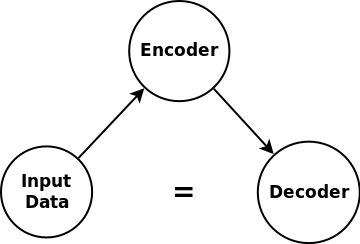
\includegraphics[width=0.5\textwidth]{pictures/figures/AE.png}
    \caption{Abstract structure of Auto-encoder}
    \label{fig:AE}
\end{figure}

To describe AE, let $\vec{X} = \{x_1, ..., x_n\} \in \mathbb{R}^n$ be input, $\vec{E} = \{e_1, ..., e_m\} \in \mathbb{R}^m$ be output from encoder layer, and $\vec{D} = \{d_1, ..., d_n\} \in \mathbb{R}^n$ be output of AE and output from decoder layer. For transform matrix, let $\bold{U}: \mathbb{R}^n \rightarrow \mathbb{R}^m$ be a transform matrix for encode layer, $\bold{V}: \mathbb{R}^m \rightarrow \mathbb{R}^n$ be a transform matrix for decode layer. The figure \ref{fig:basic_AE} describes all variables defined above.

\begin{figure}[t!]
    \centering
    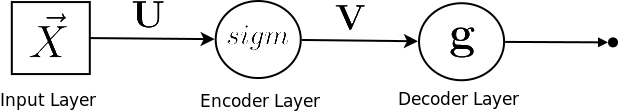
\includegraphics[width=0.5\textwidth]{pictures/figures/basic_AE.png}
    \caption{Basic Auto-encoder}
    \label{fig:basic_AE}
\end{figure}

The output of encoder is
$$\vec{E} = \bold{f}(\vec{X}\bold{U}+\vec{b_e})$$
Where $\bold{f}$ is the activation function for encoder layer and $\vec{b_e}$ is the bias for encoder layer.

The output of decoder is
$$\vec{D} = \bold{g}(\vec{E}\bold{V}+\vec{b_d})$$
Where $\bold{g}$ is the activation function for decoder layer and $\vec{b_d}$ is the bias for decoder layer.

The purpose of AE copies input as output. Therefore, cost or loss function is calculated by
$$L(\vec{X}, \vec{D}) = L(\vec{X}, \bold{g}(\bold{f}(\vec{X}\bold{U}+\vec{b_e})\bold{V}+\vec{b_d}))$$

AE seems not useful because it only tries to copy input. However, AE is usually used with other neural network and other neural network uses data from encoder layer of AE not from decoder layer. Making similar values of input and decoder output guarantees that result from encode layer contains all information of input. It means that AE can represent same information of input data in different dimension. When dimension of encoder is higher than dimension of input, it is called overcomplete Auto-encoder. When dimension of encoder is lower than dimension of input, it is called undercomplete Auto-encoder.

On this paper and experiment, undercomplete AE is used for reducing input dimension. Undercomplete AE is often compared with PCA because both methods reduce dimension. The paper \cite{hinton2006reducing} compares undercomplete AE and PCA. The result on the paper is that undercomplete AE could keep more information than PCA. It means that reducing data to low dimension by undercomplete AE gives better performance. However, training AE takes long time than computing information gain for PCA.


% When auto-encoder is traind, it has two layers: encode and decode. The encode layer receives input and passes output in lower dimension data to decode layer. The decode layer recovers dimension to input data dimention from output of encode layer. The error of auto-encoder is measured by difference between input data and output from decode layer. In other words, encoder layer compresses input data and decoder layer decompresses data from encoder layer that should be similar as original input data. That methods guarantees that the data from encoder layer keeps almost all properties of input data in lower dimension. That is the reason why output data from decode layer is similar as original input data. In math, relationship between encoder and decoder layer is similar as inverse matrix of each other.

\item Multilayer Auto-encoder\\

\end{enumerate}

\section{Deep Learning Library}\label{sec:DLL}
\subsection{DL4J}
DL4J \footnote{\url{https://deeplearning4j.org/}} is open source, distributed deep-learning library for Java and Scala. It also integrates with Hadoop and Spark. 

\subsubsection{Theano}
Theano \footnote{\url{http://deeplearning.net/software/theano/}} is a Python library for machine learning research. It integrates with Numpy and uses GPU power. The library is written in C code and optimizes user functions.

\subsubsection{Tensorflow}
Tensorflow \footnote{\url{https://www.tensorflow.org/}} is an open source software library for numerical computation using data flow graphs. The biggest difference from other libraries is that Tensorflow treats all operator as node. Another strong point is that Tesorflow allows developer to deploy computation to one or more CPUs or GPUs. 


\section{Machine Learning with Driving Data}\label{sec:MLDD}

% ####################################################################################################################################
\chapter{Data Set}
% ####################################################################################################################################


The drive simulation data is from \textit{Children's Hospital of Philadelphia} (CHOP). The simulator for the data can record 100 features with 60 samples per second from driver. The simulator has four different tracks. On the paper, the data has 16 set: 8 from expert and 8 from inexpert. Each expert and inexpert data set consist of two set of four different tracks.

% ####################################################################################################################################
\chapter{Technical Approach}
% ####################################################################################################################################

\section{Cross Validation}
There are only 16 data set. It is not enough to train neural network for general case. Whether the neural network works well on the problem or not, I used cross validation. I split 16 data set to 4 groups. Each groups have 2 expert and 2 inexpert data. The neural network is trained four times with different train (3 groups) and test (1 group) set. 

\section{LSTM}
The LSTM neural network is used to classify data because the data has time domain and LSTM neural network can handle serial data. On the paper, LSTM neural network is built with 16, 32, 64, 128, and 256 hidden neurons. The output from LSTM is sent to output layer which has two neurons. By using softmax, output from two neurons is classified. If it has [0, 1], it is classified to expert. Otherwise, it is classified to inexpert.

\begin{figure}[H]
    \centering
    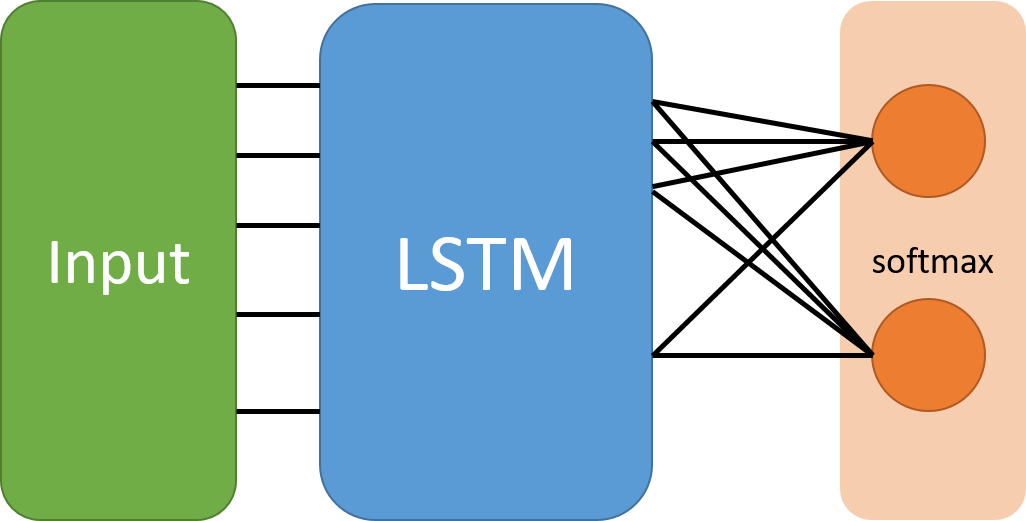
\includegraphics[width=0.5\textwidth]{pictures/applied_lstm.png}
    \caption{LSTM without Auto-Encoder}
    \label{fig:Applied LSTM}
\end{figure}

\section{Dimensionality Reduction}
The data has 100 features so dimensionality reduction is necessary. First way is selecting meaningful features and 23 features are selected. Another way to reduce dimension is auto-encoder. Before giving data to LSTM neural network, data is sent to auto-encoder layer and less dimension data from auto-encoder is sent to LSTM. 

\begin{figure}[H]
    \centering
    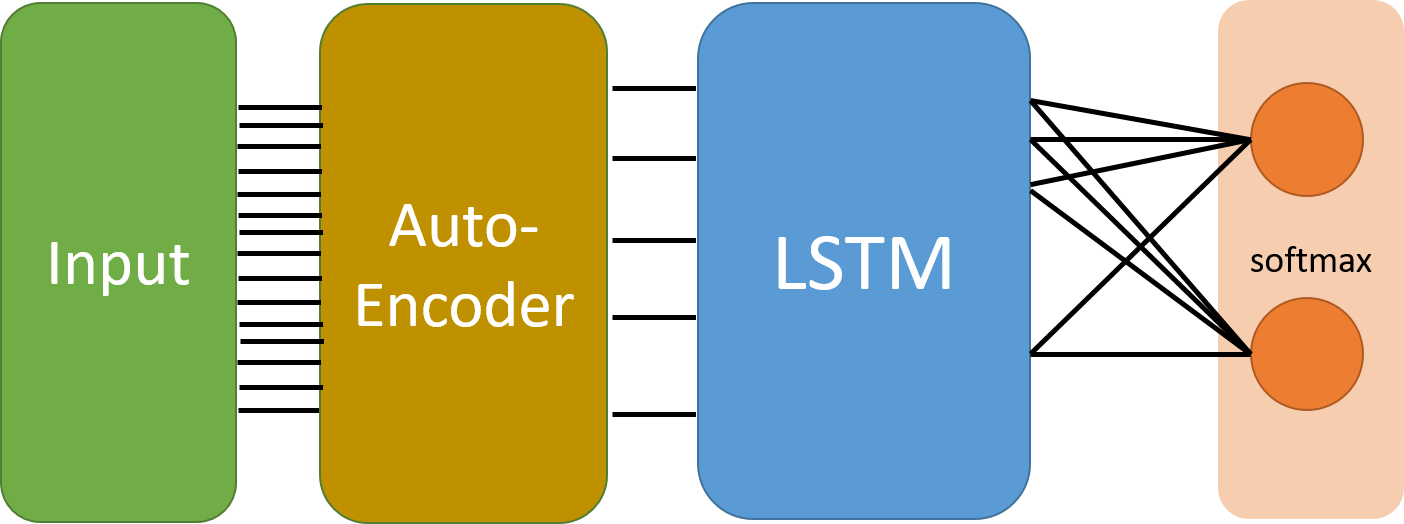
\includegraphics[width=0.5\textwidth]{pictures/applied_lstm_autoencoder.png}
    \caption{LSTM with Auto-Encoder}
    \label{fig:Applied LSTM With Auto-Encoder}
\end{figure}

%\subsection{Raw vs. Filtered data}

\section{Sampling}
The simulator records 60 samples per second. It is too often recorded. I reduce data by two way. First way is sampling one per ten and sampling one per twenty. The sampled data might not represent ten or twenty data, so average data from every ten or twenty data is used. The second way can reduce noise because there is case in first way that sampled data has more noise than other data.


% ####################################################################################################################################
\chapter{Experiment Result}
% ####################################################################################################################################


\begin{figure}[H]
    \centering
    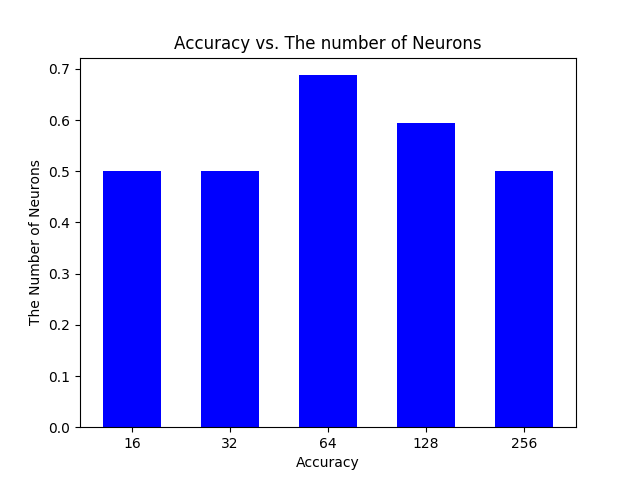
\includegraphics[width=0.75\textwidth]{pictures/accuracy.png}
    \caption{Accuracy}
    \label{fig:Accuracy}
\end{figure}


\begin{table}[H]
\centering
\begin{tabular}{|l|l|l|l|l|l|l|}
\hline
                       &      & \multicolumn{5}{l|}{The number of neurans} \\ \hline
Test                   & n    & 16    & 32    & 64      & 128      & 256   \\ \hline
\multirow{4}{*}{1}     & 1    & 0.5   & 0.25  & 1.0     & 0.5      & 0.5   \\ \cline{2-7} 
                       & 2    & 0.75  & 0.75  & 0.5     & 0.5      & 0.5   \\ \cline{2-7} 
                       & 3    & 1.0   & 0.5   & 0.5     & 0.75     & 0.5   \\ \cline{2-7} 
                       & 4    & 0.5   & 0.5   & 0.75    & 0.5      & 0.5   \\ \hline
\multirow{4}{*}{2}     & 1    & 0.5   & 0.75  & 0.75    & 0.75     & 0.75  \\ \cline{2-7} 
                       & 2    & 0.25  & 0.25  & 0.75    & 0.5      & 0.25  \\ \cline{2-7} 
                       & 3    & 0.5   & 0.5   & 0.25    & 0.75     & 0.25  \\ \cline{2-7} 
                       & 4    & 0.25  & 0.25  & 0.5     & 0.25     & 0.75  \\ \hline
\multirow{4}{*}{3}     & 1    & 0.75  & 0.25  & 1.0     & 0.75     & 0.25  \\ \cline{2-7} 
                       & 2    & 0.25  & 0.5   & 0.75    & 0.5      & 1.0   \\ \cline{2-7} 
                       & 3    & 0.5   & 0.75  & 0.75    & 0.5      & 0.5   \\ \cline{2-7} 
                       & 4    & 0.5   & 0.25  & 0.75    & 0.75     & 0.5   \\ \hline
\multirow{4}{*}{4}     & 1    & 0.75  & 0.5   & 0.5     & 0.5      & 0.5   \\ \cline{2-7} 
                       & 2    & 0.25  & 0.5   & 0.5     & 1.0      & 0.25  \\ \cline{2-7} 
                       & 3    & 0.0   & 0.75  & 1.0     & 0.75     & 0.25  \\ \cline{2-7} 
                       & 4    & 0.75  & 0.75  & 0.75    & 0.25     & 0.75  \\ \hline
\multicolumn{2}{|l|}{Average} & 0.5   & 0.5   & 0.6875  & 0.59375  & 0.5   \\ \hline
\end{tabular}
\caption{Raw 1/10 Result Summary}
\label{Raw 1/10 Result Summary}
\end{table}


% ####################################################################################################################################
\chapter{Conclusion and Future work}
% ####################################################################################################################################
Conclusion and Future work\\



\end{thesis}

\bibliography{references.bib}

\end{document}
\endinput

